\documentclass[a4paper, 11pt, oneside]{article}

\usepackage[francais]{babel}
\usepackage[utf8]{inputenc}
\usepackage{lmodern}
\usepackage[T1]{fontenc}
\usepackage{layout}

\usepackage{fancyhdr}
\usepackage{soul}
\usepackage{url}
\usepackage{listings}
\usepackage{listingsutf8}
\usepackage{geometry}
\usepackage{color}
\usepackage{graphicx}

%Pour l'espacement des paragraphes
\setlength{\parskip}{10pt plus 1pt minus 1pt}

\title{\hrule \vspace{1cm} Compte-rendu pour le TD (\no2) de l'option Sécurité Informatique}
\author{Matthias \textsc{Gradaive} - Antoine \textsc{Foucault}}
\date{\today}

\begin{document}

%Définition du style des bords de page
\pagestyle{fancy}
\lhead{}
\chead{}
\rhead{\leftmark}
\lfoot{Master 1 - ISTIC}
\cfoot{}
\rfoot{Page \thepage}

%Titre
\clearpage
\thispagestyle{empty}

\maketitle
\begin{center}
 \copyright 2014 ISTIC\\
\end{center}
\vspace{1cm}
\hrule
\thispagestyle{empty}

\newpage

%Sommaire
\renewcommand{\contentsname}{Sommaire}
\tableofcontents
\thispagestyle{empty}
\newpage
\setcounter{page}{1}

%Corps
\section*{Introduction}



\section{Questions}

\subsection{Question 1}

\subsubsection{A}

L'usage du chiffrement symétrique implique que les deux utilisateurs partagent une clé commune. Dans notre cas on a quatre utilisateurs qui veulent communiquer entre eux de façon sécurisée (chaque utilisateur veut communiquer individuellement avec un autre de façon sécurisée).\\
Ainsi, chaque utilisateur veut pouvoir communiquer avec les 3 autres de manière sécurisée. Cela implique donc 6 clés au total, pour que chaque utilisateur puisse communiquer de manière sécurisée avec les autres.

\subsubsection{B}

Il suffit de générer une paire de clé par utilisateur (donc 4 paires dans notre cas). Ainsi l'ensemble des communications est sécurisée entre chaque utilisateur.

\subsubsection{C}

Dans un système à N utilisateurs, N(N-1) clés symétriques ou N paires de clés asymétriques sont nécessaires pour assurer la confidentialité des communications entre ces utilisateurs.

\subsubsection{D}

Dans le cas de grands groupes d'utilisateurs il est préférable d'utiliser un système de chiffrement asymétrique. En effet lorsque le nombre d'utilisateurs grandit on a besoin de beaucoup plus de clés avec un système de chiffrement symétrique qu'avec un système de chiffrement asymétrique (voir questions précédente).\\
En effet pour rajouter une personne avec l'usage du chiffrement asymétrique,  il suffit seulement de lui générer une paire de clés asymétriques, lui renseigner sa clé privée et placer sa clé publique dans un annuaire par exemple. La gestion en est donc beaucoup plus simple.

\subsection{Question 2}

L'implémentation de l'algorithme DSA est effectuée dans le fichier TD.py (ne pas oublier de lire le README).\\
Les signatures produites par cet algorithme sont probabilistes. En effet, le choix de la clé éphémère k peut entraîner plusieurs signatures, et l'algorithme de vérification considère que l'ensemble de ces signatures sont correctes.

\subsubsection{A}

Après exécution de DSAVerif() avec les paramètres fournis, cette signature est correcte.

\subsubsection{B}

Après exécution de DSAVerif() avec les paramètres fournis, cette signature est incorrecte.

\newpage
\subsection{Question 3}

\subsubsection{A}

\begin{figure}[h!]
  \centering
  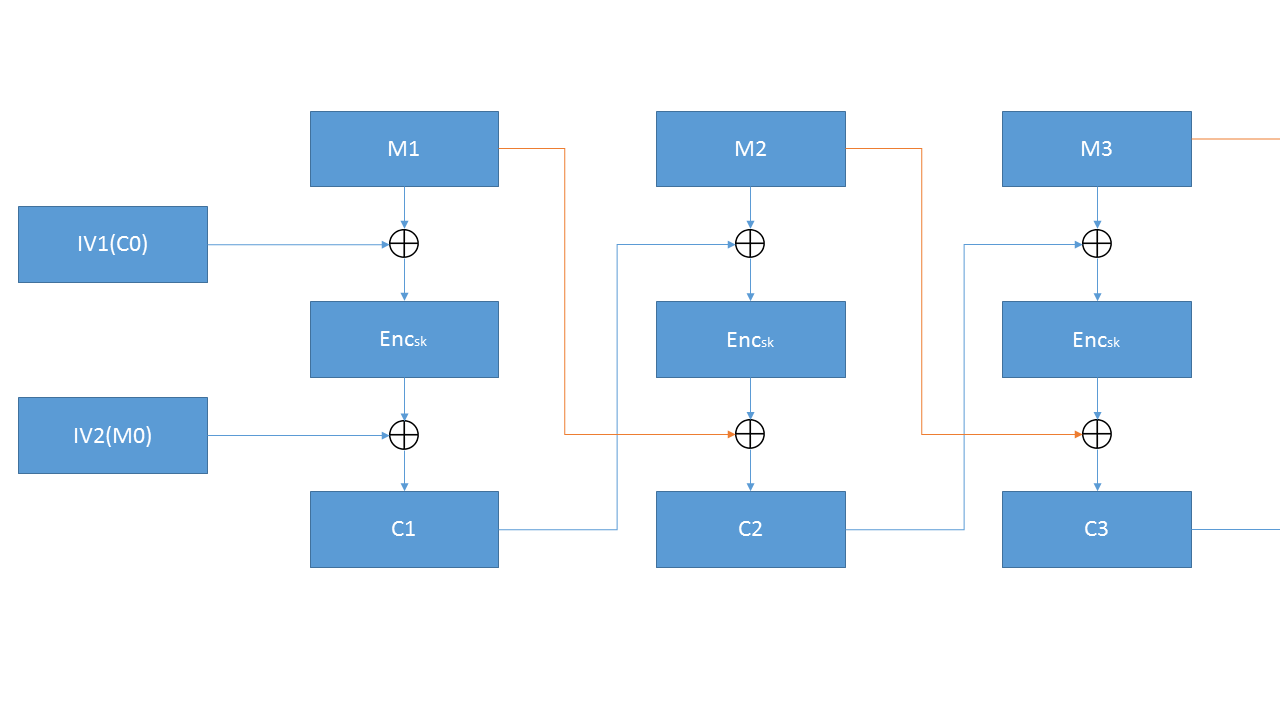
\includegraphics[width=\textwidth]{CBC.png}
  \caption{Diagramme présentant le système de chiffrement présenté dans le sujet}
\end{figure}

\subsubsection{B}

Voici la formule générale de déchiffrement d'un message : M$_{i}$ = C$_{i-1}$ XOR Dec$_{sk}$(M$_{i-1}$ XOR C$_{i}$)\\[5pt]
Pour commencer à déchiffrer le premier message (M$_{1}$), Baptiste doit avoir en sa possession les deux vecteurs d'initialisation (IV) qui sont publics. Chaque \og tour de déchiffrement \fg  permet ensuite d'obtenir l'information nécessaire au \og tour de déchiffrement \fg  suivant (Cette information est M$_{i-1}$).

\subsubsection{C}

Le sujet nous indique que le 5\ieme à été corrompu. On a donc en notre possession M5 et C5.\\
Malgrés ces informations, nous ne possédons pas la clé Sk permettant de chiffrer/déchiffrer un bloc. Par conséquent, il nous est impossible de deviner le contenu des autres blocs à partir des informations que nous possédons.

\subsubsection{D}

\subsection{Question 4}

\subsubsection{A}

Vrai. Si la taille de l’ensemble d'entrée et supérieur à l'ensemble de sortie, alors il y a obligatoirement des collisions. 

\subsubsection{B}

Vrai. Dans un protocole d’authentification, nous n'avons pas besoin de connaître l'identité de la personne. Par exemple, il suffirait d'avoir la preuve de son appartenance à un groupe qui disposent de certains droits. 

\subsubsection{C}

Ce message ne forme pas un protocole d'échange de clé sécurisé. Amélie communique seulement le hash de la clé et la signature du hash. Cela ne permet pas à Baptiste de récupérer la clé. On ne peut donc pas parler de protocole d'échange de clé.

\subsubsection{D}

Avec ne fonction de hachage à sens unique (non-cryptographique), l'engagement peut être considéré comme camouflant. En effet, l'utilisation du XOR afin de chiffrer la valeur de \textbf{i} permet à se chiffrement d'être inviolable si la valeur de \textbf{w} est aléatoire.
Par contre l'engagement n'est pas liant. La fonction de hachage n'étant pas cryptographique, il est théoriquement possible pour l’expéditeur (Alice) de calculer deux autres valeurs \textbf{x'} et \textbf{w'} tel que \textbf{H(x' XOR w') = H(x XOR w)}. 
\\[5pt]
Avec une fonction de hachage cryptographique, l'engagement est évidemment encore camouflant. De plus, Alice ne peut plus calculer de nouvelles valeurs de \textbf{x'} et \textbf{w'} tel que \textbf{H(x' XOR w') = H(x XOR w)}. L'engagement est donc à la fois liant et camouflant.

\subsection{Question 5}

Dans le système présenté pour de cette question, il serait possible pour un attaquant de deviner le contenu d'un message chiffré, la possibilité des messages clairs se résumant parfois à 2 cas. Cependant nous ne prendrons pas en compte cette remarque pour la résolution des questions.

\subsubsection{A}

Dans cette situation, Amélie doit s'assurer que son choix de restaurant ne sera pas modifié par Baptiste. Cependant ce choix n'a pas besoin d'être confidentiel.
Par conséquent, le chiffrement à clé publique n'est pas nécessaire, les destinataires doivent juste s'assurer que le message n'a pas été modifié et qu'il provient bien d'Amélie (ce qui convient exactement à l'usage d'un MAC).\\[5pt]
Amélie a donc juste à envoyer : rest$_{A}$|MAC$_{sk_{AB}}$(rest$_{A}$)|MAC$_{sk_{AC}}$(rest$_{A}$)|MAC$_{sk_{AD}}$(rest$_{A}$)\\[5pt]
Baptiste peut donc vérifier que le message provient bien d'Amélie et qu'il n'a pas été modifié. Il relaie ensuite le même message aux autres utilisateurs en enlevant sa partie MAC.
Ainsi, si Baptiste souhaite modifier le choix d'Amélie, il ne pourra pas changer les MAC destinés aux autres membres et la modification sera détectée.

\subsubsection{B}

La fête étant surprise, Baptiste ne doit pas être capable de connaître le choix de Denis. L'usage de la cryptographie asymétrique est donc justifié ici. De plus, afin d'authentifier et d'assurer l'intégrité du message, l'usage d'un MAC est également utile.\\[5pt]
Denis doit donc envoyer deux messages : 

\begin{description}
 \item[À Amélie : ] Enc$_{pk_{A}}$(rest$_{D}$)|MAC$_{sk_{AD}}$(Enc$_{pk_{A}}$(rest$_{D}$))
 \item[À Christine : ] Enc$_{pk_{C}}$(rest$_{D}$)|MAC$_{sk_{CD}}$(Enc$_{pk_{C}}$(rest$_{D}$))
\end{description}
\vspace{5pt}

De cette manière Baptiste ne peux pas lire les messages de Denis, tandis que Amélie et Christine peuvent en connaître le contenu (pour celui qui leur est adressé), ainsi qu'en vérifier l'intégrité/authenticité.

\subsubsection{C}

Dans cette situation on peut considérer Baptiste comme tiers de confiance. Baptiste va recueillir le vote de chaque membre comme un doublon de la forme [Contenu chiffré][MAC associé]. De cette manière, Baptiste est capable d'authentifier les messages qu'il reçoit, de s'assurer qu'ils n'ont pas été modifiés et d'éviter que quelqu'un vote deux fois. De plus, le chiffrement asymétrique assure que les différents votants ne connaîtront pas le choix que les autres ont pu effectuer (et ne seront pas donc influencés) avant la fin du vote.
Dans le cas où il n'y a pas chifrement asymétrique, les membres n'ont pas de moyen pour assurer la confidentialité de leurs messages. Par conséquent le mieux reste de se retrouver pour voter "physiquement" !

\subsection{Question 6}

\section*{Conclusion}



\end{document}